
In this section, we present a Lagrangian-based model capable of describing the dispersed phase with an arbitrary order of accuracy.

\subsection{Fundamental properties}

At this stage, we define some fundamental properties associated to each particle labelled $\alpha$.
Following the strategy of \citet{lhuillier2009rheology,lhuillier1992volume,zaepffel2011modelisation} and \citet[Chapter 2]{morel2015mathematical}
we define the mass $m_\alpha$, position of center of mass $\mathbf{x}_\alpha$, momentum $\textbf{p}_\alpha$ as %and total energy of the particle $\alpha$, such as,
\begin{align}
    &m_\alpha(t)
    = \int_{\Omega_\alpha(t)} \rho_2  d\Omega, \\
    % &&
    &\textbf{x}_\alpha(t)
    = \frac{1}{m_\alpha(t) }\int_{\Omega_\alpha(t)} \rho_2 \textbf{x} d\Omega, \label{eq:x_alpha}\\
    % &&
    &\textbf{p}_\alpha(t) 
    = \int_{\Omega_\alpha(t)} \rho_2 \textbf{u}_2^0 d\Omega.
    % &&
    % & m_\alpha E_\alpha(t) 
    % = \int_{\Omega_\alpha(t)} \rho_2 [e_2^0 + (u_2^0)^2/2] d\Omega,
    % \label{eq:position_and_momentum_def}
\end{align}
%respectively. 
 $\Omega_\alpha$ is the domain occupied by the particle $\alpha$ (see \ref{fig:Scheme}). 
Subsequently, we define the velocity of the particle center of mass, denoted as $\textbf{u}_\alpha$ by 
\begin{equation}
\textbf{u}_\alpha = \frac{d \textbf{x}_\alpha}{dt}  
\end{equation}
Replacing \eqref{eq:x_alpha} in the previous formula we obtain

\begin{equation}
    \textbf{u}_\alpha = \frac{1}{m_\alpha}
    \frac{d}{dt} 
    \left(
        \int_{\Omega_\alpha} \rho_2 \textbf{x} d\Omega
    \right)
    - \frac{1}{m_\alpha^2} \frac{d}{dt} \left(\int_{\Omega_\alpha} \rho_2 d\Omega \right)\int_{\Omega_\alpha} \rho_2 \textbf{x} d\Omega.
\end{equation}
%\tb{ A finaliser
Using the Reynolds transport theorem in both term in parenthesis and making use of the conservation of mass and definition \eqref{eq:x_alpha} in the last term

\begin{equation}
    \textbf{u}_\alpha = \frac{1}{m_\alpha}\int_{\Omega_\alpha} \left[
        \pddt (\rho_2 \textbf{x}) + \div\left(\rho_2 \textbf{x}\textbf{u}_2\right) 
    \right]d\Omega \\
    + \frac{1}{m_\alpha}\int_{\Sigma_\alpha} \textbf{x} \rho_2(\textbf{u}_I   - \textbf{u}_2) \cdot \textbf{n}_2 d \Sigma
    -  \frac{\textbf{x}_\alpha}{m_\alpha}    \int_{\Sigma_\alpha} \rho_2(\textbf{u}_I   - \textbf{u}_2) \cdot \textbf{n}_2 d\Sigma 
\end{equation}
Then by considering the mass conservation for the first term, noticing that $\grad \textbf{y} = \bm\delta$ where $\bm\delta$ is the identity tensor for the second term, and introducing $\mathbf{r} = \mathbf{y} - \mathbf{y}_\alpha$ for the last two terms gives, 
%\begin{equation}
%    \textbf{u}_\alpha = \frac{1}{m_\alpha}\int_{\Omega_\alpha} \textbf{x} \left[
%    \pddt (\rho_2) + \div\left(\rho_2 \textbf{u}_2\right) 
%    \right]d\Omega
%    + \frac{1}{m_\alpha}\int_{\Omega_\alpha} \rho_2  \textbf{u}_2  \cdot \grad \textbf{x} d\Omega \\
%    &+ \frac{1}{m_\alpha}\int_{\Sigma_\alpha} \textbf{x}_2 \rho_2 (\textbf{u}_I - \textbf{u}_2) \cdot \textbf{n}_2 d \Sigma
%    - \frac{1}{m_\alpha}  \textbf{x}_\alpha \int_{\Sigma_\alpha} \rho_2(\textbf{u}_I   - \textbf{u}_2) \cdot \textbf{n}_2 d\Sigma
%\end{equation}

%}
%The derivation of $\ddt {\textbf{x}_\alpha}$ is straightforward but requires some algebra which are detailed in \ref{ap:velocity_definition}. 
%The final expression reads,
\begin{equation}
    \textbf{u}_\alpha(t) = \frac{1}{m_\alpha(t)} \left(
        \textbf{p}_\alpha(t)
        +  \int_{\Sigma_\alpha(t)} \rho_2 \textbf{r} (\textbf{u}_I^0 - \textbf{u}_2^0)\cdot \textbf{n}_2 d\Sigma
        \right),
        \label{eq:dt_y_alpha}
\end{equation}
where $\textbf{r}(\textbf{x},t) = \textbf{x} - \textbf{x}_\alpha(t)$. 
In Equation \ref{eq:dt_y_alpha}, it can be observed that the first component of the velocity represents the linear momentum divided by the mass of the particle. 
This corresponds to the mass-averaged velocity over the volume of the particle.
The second term in Equation \ref{eq:dt_y_alpha} arises from the contribution of anisotropic mass transfer across the surface of the particle. 
This mass transfer leads to the motion of the particle's center of mass, thereby contributing to the total velocity.
To illustrate this concept, let us consider a fixed drop with no momentum lying over a very hot plate.
In this scenario, we assume that the plate is sufficiently hot to induce evaporation, specifically on the bottom portion of the drop.
Hence, under the effect of an anisotropic evaporation flux one may expect the second term to be non-negligible.
Consequently, the center of mass of the drop has a non-zero velocity in the opposite direction of the plate, even though the momentum is assumed to be zero.
% We can also consider the case of the nucleation of a bubble in water. 
% In this case, although the particle momentum is null at all time the center of mass of the particle moves due to the growth of the particle. 
% In both cases, we need to take into account the mass transfer term in \ref{eq:dt_y_alpha}, while the first term is negligible. 
Note that \ref{eq:dt_y_alpha} generalized usual expression of the center of mass velocity whom neglect the second term.
In the following, for the sake of brevity we discard the time dependency notation for all Lagrangian quantities denoted by the subscript $_\alpha$ and in particular $\Sigma(t)$ and $\Omega_\alpha$.
Nevertheless, the reader must understand that all Lagrangian quantities and integration domains subscribed by $_\alpha$ are time dependent. 

The particle's internal relative motions or the \textit{inner velocity} is given by $\textbf{w}_2^0(\textbf{x},t) = \textbf{u}_2^0(\textbf{x}) - \textbf{u}_\alpha(t)$. Then the momentum of the particle reads
%Thus, from its definition in \ref{eq:position_and_momentum_def}, we can rewrite the momentum as follows,
\begin{equation}
    \label{eq:momentum_definition_1}
    \textbf{p}_\alpha
    = m_\alpha \textbf{u}_\alpha
    + \int_{\Omega_\alpha} \rho_2 \textbf{w}_2^0 d\Omega.
\end{equation}
Alternatively, from \eqref{eq:dt_y_alpha}, we obtain,
\begin{equation}
    \textbf{p}_\alpha
    =  m_\alpha \textbf{u}_\alpha
    - \int_{\Sigma_\alpha} \rho_2\textbf{r}(\textbf{u}_I^0 - \textbf{u}_2^0)\cdot \textbf{n}_2 d\Sigma
    \label{eq:momentum_definition}
\end{equation}
Therefore, the momentum of a particle can be seen as a sum of the mean velocity plus the integral of the fluctuation (\ref{eq:momentum_definition_1}), with the latter being equivalent to minus the first moment of mass transfer term (\ref{eq:momentum_definition}).
Indeed, by identification we obtain : $\int_{\Omega_\alpha} \rho_2 \textbf{w}_2^0 d\Omega =\int_{\Sigma_\alpha}  \rho_2\textbf{r} (\textbf{u}_I^0 - \textbf{u}_2^0)\cdot \textbf{n}_2 d\Sigma$. 
%The essential aspect of this relation highlighted here is that 
Hence the internal velocity fluctuations within a fluid particle do not contribute to the total linear momentum $\textbf{p}_\alpha$, as long as the anisotropic mass transfer is negligible.  
% Additionally, the total energy $E_\alpha$ can be decomposed following a similar procedure which leads us to, 
% \begin{equation*}
%     \label{eq:E_alpha_def}
%     m_\alpha E_\alpha(t) 
%     = m_\alpha e_\alpha 
%     + W_\alpha
%     + m_\alpha (u_\alpha)^2/2
%     % + \textbf{u}_\alpha \cdot \int_{\Omega_\alpha(t)} \rho_2  \textbf{w}_2^0 d\Omega
% \end{equation*}
% where we introduced the internal kinetic energy : $W_\alpha = \int_{\Omega_\alpha(t)} \rho_2  (w_2^0)^2/2 d\Omega$. 
% In that expression mass transfer have been neglected. 
% The total energy of a particle is the sum of its internal energy $e_\alpha$, internal kinetic energy $W_\alpha$ and the kinetic energy  due to its own center of mass displacement $u_\alpha^2/2$. 
% To gain in understanding, let's express $W_\alpha$ in the case of a solid particle.
% The velocity inside a solid particle can be expressed : $\textbf{u}_2^0(\textbf{x}_\alpha + \textbf{r}) = \textbf{u}_\alpha + \textbf{r}\times \bm{\omega}_\alpha$ where $\bm{\omega}_\alpha$ is the angular velocity.  
% In this case, $W_\alpha = \bm{\omega}_\alpha\bm{\omega}_\alpha\cdot \\bm\delta_\alpha$ where $\\bm\delta_\alpha$ is the inertia matrices of the particle. 
% As a matter of facts for solid particles $W_\alpha$ represents the angular kinetic energy for solid particles.
% Thus, for particles with fluid internal motion, $W_\alpha$ is just a more general definition of the particle internal kinetic energy. 

\subsection{Conservation laws}

We assign to a particle indexed, $\alpha$, occupying the domain $\Omega_\alpha$ (see \ref{fig:Scheme}) an arbitrary Lagrangian property $q_\alpha$ defined by $q_\alpha  = \intO{ f_2^0(\textbf{x},t) }$.
Similarly, we define $q_{I\alpha} = \intS{ f_I^0(\textbf{x},t) }$ as being an integrated surface property associated to the particle $\alpha$.
%\tb{mettre + de detail avec les theorem}
To describe the evolution of any arbitrary Lagrangian quantity $q_\alpha$, we need to establish its time derivative.
Since, $q_\alpha$ is an integral quantity with a time-dependent domain of integration, we apply the general Reynolds transport theorem for volume integral (exposed in \ref{ap:math}) to compute its time derivative \citep{morel2015mathematical}.
This yields the following expression :
\begin{equation}
    \ddt  q_\alpha
    = \intO{\left[ \pddt f_2^0 + \div\left(f_2^0\textbf{u}_2^0\right) \right]}\\
    + \intS{ f_2^0 (\textbf{u}_I^0-\textbf{u}_2^0)\cdot \textbf{n}_2 }.
\end{equation}
By substituting the integrand of the first integral on the right-hand side (RHS) with \ref{eq:dt_f_k} and making use of the divergence theorem we obtain the conservation laws of the quantity $q_\alpha$, namely,  
\begin{equation}
    \ddt  q_\alpha
    = \intO{ s_2^0 }
    + \intS{ \left[
        f_2^0 (\textbf{u}_I^0-\textbf{u}_2^0) 
        + \mathbf{\Phi}_2^0 
        \right] \cdot \textbf{n}_2 },
    \label{eq:dt_q_alpha}
\end{equation}
The first term on the right-hand side accounts for the total contribution of the source term $s_2^0$ to the particle $\alpha$.
While, The second term on the right-hand side is the surface integration of the exchange terms, which includes the phase transfer flux $f_2^0 (\textbf{u}_I^0-\textbf{u}_2^0)$ and the diffusive flux $\mathbf{\Phi}_2^0$. 


\tb{a mettre apres les considerations sur les surfaces or not ?  }
Let us consider the specific case of the momentum balance, i.e. $q_\alpha = \textbf{p}_\alpha$.
In this situation, equation \eqref{eq:dt_q_alpha} reads
\begin{equation}
    \ddt  \textbf{p}_\alpha
    = \intO{ \rho_2\textbf{g} }
    + \intS{ \left[
        f_2^0 (\textbf{u}_I^0-\textbf{u}_2^0)
        + \bm{\sigma}_2^0%\cdot\textbf{n}_2  
        %+ \mathbf{\Phi}_2^0 
        \right] \cdot \textbf{n}_2 },
    \label{eq:dt_q_alpha}
\end{equation}

% first term reads as $\intO{ \rho_2\textbf{g} }$ 
The first term on the right-hand side represents the total weight acting on the particle $\alpha$, the second term represents the total source of momentum due to phase transfer, and it is expressed as, $\intS{ \rho_2 \textbf{u}_2^0 (\textbf{u}_I^0-\textbf{u}_2^0)\cdot\textbf{n}_2 }$. 
Lastly, $\intS{ \bm{\sigma}_2^0\cdot\textbf{n}_2 }$ represents the resultant of the hydrodynamic forces acting on the surface of the particle.
It is important to notice that under this form, the exchange terms are expressed as integrals of dispersed phase fields denoted by the subscript $_2$.
Nevertheless, depending on the nature of the dispersed phase, these fields may not always be defined.
For rigid particles the stress within the particle $\bm{\sigma}_2^0$ is not indeterminate \citep{guazzelli2011}.  
Hence, our objective is to express these exchange terms, in terms of the continuous phase field quantities instead of the dispersed phase field, i.e. in terms of $\mathbf{\Phi}_1^0$ and $\textbf{u}_1^0$ rather than $\mathbf{\Phi}_2^0$ and $\textbf{u}_2^0$. 

To address this issue, let us derive the conservation equation for the integrated surface property $q_{I\alpha}$.
To differentiate time-varying surface integrals within time, we can use the general Leibniz rule (see \ref{eq:Leibnitz}), to derive the following expression
\begin{equation}
    \ddt  q_{I\alpha}
    = \intS{ \left[
        \pddt f_I^0
        +   \gradI \cdot (\textbf{u}_I^0f_I^0)
    \right]}.
    \label{eq:surface_derivative}
\end{equation}
%Substituting the RHS terms of \ref{eq:surface_derivative} 
Using \ref{eq:dt_f_I} and the surface divergence theorem on closed surfaces (see \ref{eq:surf_div_theorem}), gives,
\begin{equation}
    \ddt  q_{I\alpha}
    = \intS{ 
        s_I^0
    }
    - \intS{
\sum_k \left[
    f_k^0 (\textbf{u}_I^0 - \textbf{u}_k^0)
    + \mathbf{\Phi}_k^0
    \right] \cdot \textbf{n}_k 
 %\Jump{
        %f_k^0 (\textbf{u}_I^0 - \textbf{u}_k^0)
        %+ \mathbf{\Phi}_k^0
    %}
    }.
    \label{eq:dt_q_I_alpha}
\end{equation}
This equation can be interpreted as the surface conservation equation for the integrated surface property $f_I$, or as the flux jump condition integrated on a closed surface. Notice that $\bm{\Phi}_{I}^0$ is not present in this balance equation. 
This is due to the fact that as mentioned earlier, only the tangential components of $\bm{\Phi}_{I}^0$ appear inside the surface balance equation, while we perform an integration over a closed surface which is null due to \ref{eq:surf_div_theorem}. As discussed above we wish to get rid of $\mathbf{\Phi}_2^0$ in \ref{eq:dt_q_alpha}. To achieve this, we treat the particle's volume and surface as a unified entity and derive a conservation equation for $q_\alpha^\text{tot} = q_\alpha + q_{I\alpha}$. 
This is done by summing \ref{eq:dt_q_alpha} and \ref{eq:dt_q_I_alpha} which leads to, 
\begin{equation}
    \ddt  q_\alpha^\text{tot}
    = 
    \intO{ s_2^0 }
    + \intS{ s_I^0 }
    + \intS{ \left[
        f_1^0 (\textbf{u}_I^0-\textbf{u}_1^0) 
        + \mathbf{\Phi}_1^0 
        \right] \cdot \textbf{n}_2 }. 
    \label{eq:dt_q_alpha_tot}
\end{equation}
This equation is the general form of the linear conservation law for the quantity $q_\alpha^\text{tot}$. %of $\chi_2 f_2^0 + \delta_I f_I^0$ for the system consisting of the particle volume $\Omega_\alpha$, and its surface $\Sigma_\alpha$. 
It is applicable to any particle immersed into a continuous phase following the local conservation,\ref{eq:dt_f_k} and \ref{eq:dt_f_I}.
We refer to this equation as the zeroth-order conservation equation or the linear conservation law for the particle $\alpha$.

% Following the same assumption as in \ref{sec:local_eq}, i.e. we consider no mass transfer and weightless interfaces, the Lagrangian  mass, momentum and energy equations for a single particle can be derived using the generic form \ref{eq:dt_q_alpha_tot} and reads as, 
% \begin{align}
%     \label{eq:dt_m_alpha}
%     \ddt m_\alpha
%     &= 
%     0\\
%     \label{eq:dt_p_alpha}
%     \ddt (m_\alpha \textbf{u}_\alpha)
%     &= 
%     m_\alpha\textbf{g}
%     +  \intS{\bm{\sigma}_1^0 \cdot \textbf{n}_2}\\
%     \label{eq:dt_E_alpha}
%     \ddt (m_\alpha E_\alpha + s_\alpha \gamma)
%     &= 
%     m_\alpha \textbf{u}_\alpha \cdot \textbf{g}
%     +\textbf{u}_\alpha \cdot \intS{\bm{\sigma}_1^0 \cdot \textbf{n}_2}
%     +\intS{\textbf{w}_1^0 \cdot \bm{\sigma}_1^0 \cdot  \textbf{n}_2} 
%     - \intS{\textbf{q}_1^0 \cdot \textbf{n}_2}
% \end{align}
% where  $\intS{  \bm{\sigma}_1^0 \cdot \textbf{n}_2 }$ is the resultants of the hydrodynamic force and $\intS{ \textbf{q}_1^0 \cdot \textbf{n}_2 }$ is the resultants of the surface heat flux. 
% The second term on the right-hands side of the energy equation is the work produced by the mean force and the translational motion of the droplets, while $\intS{\textbf{w}_1^0 \cdot \bm{\sigma}_1^0 \cdot  \textbf{n}_2}$ is the work produced by the local forces and local motion of the fluid at the surface of the particle.
% Since we integrated the energy over the particle's volume and its surface, we explicitly made appear the surface energy $\gamma s_\alpha$ within the derivative operator. 
% Note that these equations does not explicitly account for inter-particle interactions. 
% However, it is possible to include manually such forces by noticing that the surface external stress flux $\bm{\sigma}_1^0$ is the sum of hydrodynamic and particles-particles interaction forces, regardless it is pure contact forces from direct contact or a force mediated through the carrier fluid.
% From this consideration it is possible to split every term involving the stress $\bm{\sigma}_1^0$ into two terms representing these contributions. 
% Same comments can be made for the heat flux $\textbf{q}_1^0$. 
% Although this distinction is important, for purpose of clearly we will stay general, and we will keep the fluxes $\bm{\sigma}_1^0$ and $\textbf{q}_1^0$ as such. 

% In the spirit of the energy decomposition exposed in \ref{eq:E_alpha_def} the total energy equation can be split into three equations, one for the center of mass kinetic energy, internal motion and internal kinetic energy, namely,  
% \begin{align}
%     \label{eq:dt_u2_alpha}
%     \frac{1}{2}\ddt (m_\alpha u_\alpha^2)
%     &= 
%     \textbf{u}_\alpha\cdot
%     \textbf{g}m_\alpha
%     + 
%     \textbf{u}_\alpha\cdot
%     \textbf{f}_\alpha,\\
%     \label{eq:dt_w2_alpha}
%     \ddt (W_\alpha + \gamma s_\alpha)
%     &= 
%     \intS {\textbf{w}_1^0 \cdot \bm{\sigma}_1^0 \cdot \textbf{n}_2 }
%     - \intO{ \bm{\sigma}_2^0 : \grad\textbf{u}_2^0 }
%     \\
%      \label{eq:dt_e_alpha}
%     \ddt (m_\alpha e_\alpha )
%     &= 
%      \intO{ \bm{\sigma}_2^0 : \grad\textbf{u}_2^0  }
%     -  \intS{\textbf{q}_1^0\cdot \textbf{n}_2 } 
% \end{align}
% respectively. 
% Note that in \citet{eq:dt_w2_alpha} the use of \ref{eq:dt_rhoI_uI2} makes appear explicitly the derivative of the surface energy $s_\alpha \gamma$. 
% Note that under this form we see that the energy loss in the deformation represented by $W_p$ will be gathered in the surface energy which will in turn act as a source term in the internal kinetic energy motion.
% The surface tension plays the role as a spring in the energy balance.   
% From this set of equation we can easily see that the rate of dissipation terms $\intS{\bm{\sigma}_2^0 : \grad\textbf{u}_2^0}$ represent an energy sink in the equation of $W_\alpha$ while it is a source term in the internal energy equation. 
% As it has been observed in the previous section, this terms convert the energy of internal motion to molecular agitation. 
% However, the interplay between the center of mass  kinetic energy and the internal fluctuation is not obvious and has no common term with the heat and internal kinetic energy equation.
% In fact, we will see that the transfer between these scales is archived thought the fluid phase pseudo turbulent energy. 


Finally, we would like to highlight that  due to the consideration of closed surface, the diffusive flux $\mathbf{\Phi}_I$, plays no role at all in \ref{eq:dt_q_alpha_tot}.
Therefore, in the case of the linear momentum conservation law, the contribution of the surface tension forces exposed in \ref{eq:surface_tension}, do not contribute to the momentum balance in \ref{eq:dt_p_alpha}.
As a consequence, even in the presence of local Marangoni forces, the resultant of the local surface tension forces would cancels out in the linear momentum balance.
This fact has already been demonstrated by \citet{hesla1993note} who showed that the surface tension force does not contribute to the linear and angular momentum balance. 
Here, we have provided the general proof that the interfacial diffusive flux $\mathbf{\Phi}_I^0$, which is present at the local scale according to \ref{eq:dt_f_I}, does not contribute to the zeroth-order conservation law of a particle with a closed surface.

\subsection{Moment equations}

Because $f_2^0$ and $f_I^0$ are not constant inside each particle's volume, it is interesting to introduce in the first place, the the first moment of the quantities $f_2^0$ and $f_I^0$. 
They are defined as
\begin{align}
    &\textbf{Q}_\alpha 
    = \intO{ \textbf{r} f_2^0 },
    &\text{and}&
    &\textbf{Q}_{I\alpha}
    = \intS{ \textbf{r} f_I^0 },
    \label{eq:first_moment_definition}
\end{align}
where we recall that $\textbf{r} = \textbf{x} - \textbf{x}_\alpha$ is the distance between any point inside $\Omega_\alpha$ or $\Sigma_\alpha$, to the center of mass of the particle $\alpha$.
It is then possible to differentiate these moments with respect to time in order to obtain their conservation laws.
%In this appendix we propose a detailed derivation of the moments equations. 
%The first moment or dipoles of any property $q_\alpha$ can be defined as,
%\begin{equation*}
%    \textbf{Q}_\alpha 
%    = \int_{\Omega_\alpha} \textbf{r} f_2 d\Omega
%\end{equation*}
We use the Reynolds transport theorem to describe the evolution of $\textbf{Q}_\alpha$ within time. 
It gives, 
\begin{equation}
    \frac{d}{dt} \textbf{Q}_\alpha
      =  \int_{\Omega_\alpha} \left[
        \pddt(\textbf{r}  f_2^0)
        + \div \left( \textbf{r} f_2^0 \textbf{u}_2^0\right)
    \right]d\Omega + \int_{\Sigma_\alpha} \textbf{r}  f_2^0  (\textbf{u}_I^0-\textbf{u}_2^0)\cdot \textbf{n}_2  d\Sigma  \nonumber
%    &=  \int_{\Omega_\alpha} \textbf{r}\left[
%        \pddt f_2^0
%        + \div \left(f_2^0 \textbf{u}_2^0\right)
%    \right] d\Omega
%    + \int_{\Omega_\alpha} f_2^0 \left[
%        \pddt \textbf{r}
%        +\textbf{u}_2^0 \grad \textbf{r}
%    \right]d\Omega\\
%    &+ \int_{\Sigma_\alpha} \textbf{r}  f_2^0 (\textbf{u}_I^0-\textbf{u}_2^0)\cdot \textbf{n}_2  d\Sigma,
\end{equation}
The first term on the right-hand side may be rewritten as
\begin{equation}
\int_{\Omega_\alpha} \left[
        \pddt(\textbf{r}  f_2^0)+ \div \left(f \textbf{r} \textbf{u}_2^0\right) 
    \right]d\Omega
    = \int_{\Omega_\alpha} \textbf{r}\left[
        \pddt f_2^0
        + \div \left(f_2^0 \textbf{u}_2^0\right)
    \right] d\Omega
    + \int_{\Omega_\alpha} f_2^0 \left[
        \pddt \textbf{r}
        +\textbf{u}_2^0 \cdot \grad \textbf{r}
    \right]d\Omega
\end{equation}
Using \ref{eq:dt_f_k} for the first term appearing on the right-hand side of the previous equation, and considering the relation,
$  \pddt \textbf{r}
+ \textbf{u}_2^0 \cdot \grad \textbf{r}
= - \frac{d}{dt} \textbf{y}_\alpha  + \textbf{u}_2^0 \cdot \bm\delta
= \textbf{w}_2$,
for the second term yields the relation,
\begin{align*}
    \frac{d}{dt} \textbf{Q}_\alpha
    &= \int_{\Omega_\alpha} \textbf{r} \left[
         \textbf{S}_2 +  \div \mathbf{\Phi}_2
    \right]d\Omega
    +\int_{\Omega_\alpha} f_2^0  \textbf{w}_2 d\Omega
    + \int_{\Sigma_\alpha} \textbf{r}  f_2^0 (\textbf{u}_I^0-\textbf{u}_2^0)\cdot \textbf{n}_2  d\Sigma,\\
    &= \int_{\Omega_\alpha} \left( 
        \textbf{r} \textbf{S}_2 
        - \mathbf{\Phi}_2
        + f_2^0  \textbf{w}_2 
    \right) d\Omega
    + \int_{\Sigma_\alpha} \textbf{r} \left[
        \mathbf{\Phi}_2
        + f_2^0 (\textbf{u}_I^0-\textbf{u}_2^0)
    \right]\cdot \textbf{n}_2  d\Sigma.
\end{align*}
To pass from the first line to the second lines we noticed that $\int_{\Omega_\alpha} \textbf{r}  \div \mathbf{\Phi}_2 d\Omega
= \int_{\Sigma_\alpha} \textbf{r} \mathbf{\Phi}_2 \cdot \textbf{n}_2 d\Sigma
- \int_{\Omega_\alpha} \mathbf{\Phi}_2 d\Omega$. 
% \JL{Dans le corps du texte tu notes $d\Sigma$ et $d\Omega$ les differentielles des surfaces et des volumes. Merci de faire la meme chose en annexe. Par ailleurs je trouve qu'il manque des explications pour passser de 78 a 79 (j'imagine que tu utilises la conservation du moment d'ordre 0) et pour passer de 79 a 80 ou tu dois faire une integration part partie. Encore faut il le preciser ...}





Indeed, considering \ref{eq:dt_f_k}, \ref{eq:dt_f_I} and applying the Leibniz rule for volume and surface integrals (see \ref{eq:Reynolds} and \ref{eq:Leibnitz} respectively), we can show equally that,
\begin{align}
    \ddt {\textbf{Q}_\alpha}
    &= \intO{ \left(
        \textbf{r} s_2^0         
        + f_2^0  \textbf{w}_2^0 
        - \mathbf{\Phi}_2^0
    \right) },
    + \intS{ \textbf{r} \left[
        \mathbf{\Phi}_2^0
        + f_2^0 (\textbf{u}_I^0-\textbf{u}_2^0)
    \right]\cdot \textbf{n}_2  } 
    \label{eq:dt_Q_alpha}\\
    \ddt {\textbf{Q}_{I\alpha}}
    &= \intS{ \left(
        \textbf{r}s_I^0
        + f_I^0 \textbf{w}_I^0
        - \mathbf{\Phi}_{I||}^0
    \right) },
    - \intS{\textbf{r} 
    \Jump{\mathbf{\Phi}_k^0
        + f_k^0 (\textbf{u}_I^0 - \textbf{u}_k^0)
    }
    },
    \label{eq:dt_Q_I_alpha}
\end{align}
where $\textbf{w}_I^0 = \textbf{u}_I^0 - \textbf{u}_\alpha$.
The detailed derivation of \ref{eq:dt_Q_alpha} is provided in \ref{ap:moment_derivative}.
The derivation of \ref{eq:dt_Q_I_alpha} follows a similar procedure. 
In \ref{eq:dt_Q_alpha}, we recognize the first moment of the source term $s_2^0$, the first moment of the diffusive flux term $\mathbf{\Phi}_2^0\cdot\textbf{n}_2$ and the first moment of phase exchange term, $f_2^0 (\textbf{u}_I^0-\textbf{u}_2^0)\cdot\textbf{n}_2$. 
Additionally, two supplementary terms appear in \ref{eq:dt_Q_alpha}, namely : the integral of the diffusive flux $\mathbf{\Phi}_2^0$, and a term related to the fluctuation of the internal velocity $f_2^0 \textbf{w}_2^0$.
Similar observations can be made for the fist moment of surface equation \ref{eq:dt_Q_I_alpha}, as it shares similarities with \ref{eq:dt_Q_alpha}. 
In particular, it is worth noting the presence of the surface diffusive flux $\mathbf{\Phi}_{I||}^0$ in \ref{eq:dt_Q_I_alpha}.
This term will be further discussed and analyzed in the following. 

For similar reason than the linear conservation equations, we sum \ref{eq:dt_Q_alpha} and \ref{eq:dt_Q_I_alpha} to expresses the conservation equation of the total first moment $\textbf{Q}_\alpha^\text{tot} = \textbf{Q}_\alpha + \textbf{Q}_{I\alpha}$.
This leads to the following expression:
\begin{multline}
    \ddt {\textbf{Q}_\alpha^\text{tot}}
    = \intO{ \left(
        \textbf{r} s_2^0         
        + f_2^0  \textbf{w}_2^0 
        - \mathbf{\Phi}_2^0
    \right) }
    + \intS{ \left(
        \textbf{r}s_I^0
        + f_I^0 \textbf{w}_I^0
        - \mathbf{\Phi}_{I||}^0
    \right) }
    + \intS{ \textbf{r} \left[
        \mathbf{\Phi}_1^0
        + f_1^0 (\textbf{u}_I^0-\textbf{u}_1^0)
    \right]\cdot \textbf{n}_2  }. 
    \label{eq:dt_Q_alpha_tot}
\end{multline}
Likewise, conservation laws can be derived for an arbitrary $n^{th}$ order moments of volume and surface, i.e. for
\begin{align}
    \textbf{Q}_\alpha^n
    = \intO{
         \underbrace{\textbf{rr}\ldots \textbf{rr}}_{n\text{ times}}
        f_2^0 },
        && \text{and} &&
    \textbf{Q}_{I\alpha}^n
    = \intS{
         \underbrace{\textbf{rr}\ldots \textbf{rr}}_{n\text{ times}}
    f_I^0 },
    \label{eq:Q_n_definition}
\end{align} 
respectively. 
It can be shown that the derivative with time of do not involve any additional terms than in \ref{eq:dt_Q_alpha} and \ref{eq:dt_Q_I_alpha}, but rather just the $n^{th}$ order moments of the already presented terms.
We provide the full derivation of $\ddt{ \textbf{Q}_\alpha^n}$ in \ref{ap:Moments_equations}.
In short, these higher order moments describe the distributions of the local quantities $f_2^0$ and $f_I^0$ inside the domain $\Omega_\alpha$ and $\Sigma$ respectively.
Consequently, an infinite number of moments would be theoretically necessary to recover the fields of $f_2^0$ and $f_I^0$  within $\Omega_\alpha$ and $\Sigma$. 

\tb{Disscusion on Marangoni stresses ?}
\subsubsection{Discussion}

To gain physical insight in the meaning the moments equations we consider the second order moment of mass and first order moment of momentum.
Following \ref{eq:Q_n_definition} we define the second-order moment of mass and the first-order moment of momentum as respectively,
\begin{equation}
    \textbf{M}_\alpha 
    = \intO{ \rho_2 \textbf{r} \textbf{r} }
    \;\;\;\text{and}\;\;\;
    \textbf{P}_\alpha 
    = \intO{ \rho_2 \textbf{r} \textbf{u}_2^0 }.
    \label{eq:first_moment_of_momentum_def}
\end{equation}
Note that $\textbf{M}_\alpha$ is analogous to the inertia tensor $\textbf{I}_\alpha$ in solid mechanics, and they are related through the expression, $\textbf{I}_\alpha = \text{tr}(\textbf{M}_\alpha)\bm\delta - \textbf{M}_\alpha$.
For a constant density the tensor $\textbf{M}_\alpha$ describes the second moment of the volume distribution around the particle center of mass.
In order to provide a clearer physical interpretation to the moment of momentum tensor, we decompose $\textbf{P}_\alpha$ into two distinct part, namely,
$\textbf{P}_\alpha = \textbf{S}_\alpha+\textbf{T}_\alpha$ where $\textbf{S}_\alpha$ represents the symmetric part and $\textbf{T}_\alpha$ is the antisymmetric part of $\textbf{P}_\alpha$.
The tensors $\textbf{S}_\alpha$ and $\textbf{T}_\alpha$ correspond respectively to the stretching and angular momentum of the particle $\alpha$. 
The tensor $\textbf{S}_\alpha$ quantifies how fast and in which direction the particle get elongated or flattened, in other worlds it represents the rate of deformation experienced by the particle.
The tensor $\textbf{T}_\alpha$ is related to the angular momentum of the particle. 
In this study we use the pseudo vector $\bm{\mu}_\alpha = \intO{ \rho_2 \textbf{r} \times \textbf{u}_2^0 }$ to express this quantity. 
Indeed, both  $\textbf{T}_\alpha$ and $\bm{\mu}_\alpha$ represent the angular momentum and are related through $(\bm{\mu}_\alpha)_i = \epsilon_{ijk} (\textbf{P}_\alpha)_{jk}= \epsilon_{ijk} (\textbf{T}_\alpha)_{jk}$, where $\bm\epsilon$ is the third order alternating unit tensor, or Levi-Cita tensor. 
Lastly, we also introduce the scalar $D_\alpha = \text{tr}(\textbf{P}_\alpha) = \frac{1}{3}\intO{ \rho_2 \textbf{r} \cdot \textbf{u}_2^0 }.$, which quantifies the rate at which the particle is being compressed.

\begin{figure}
    \centering
    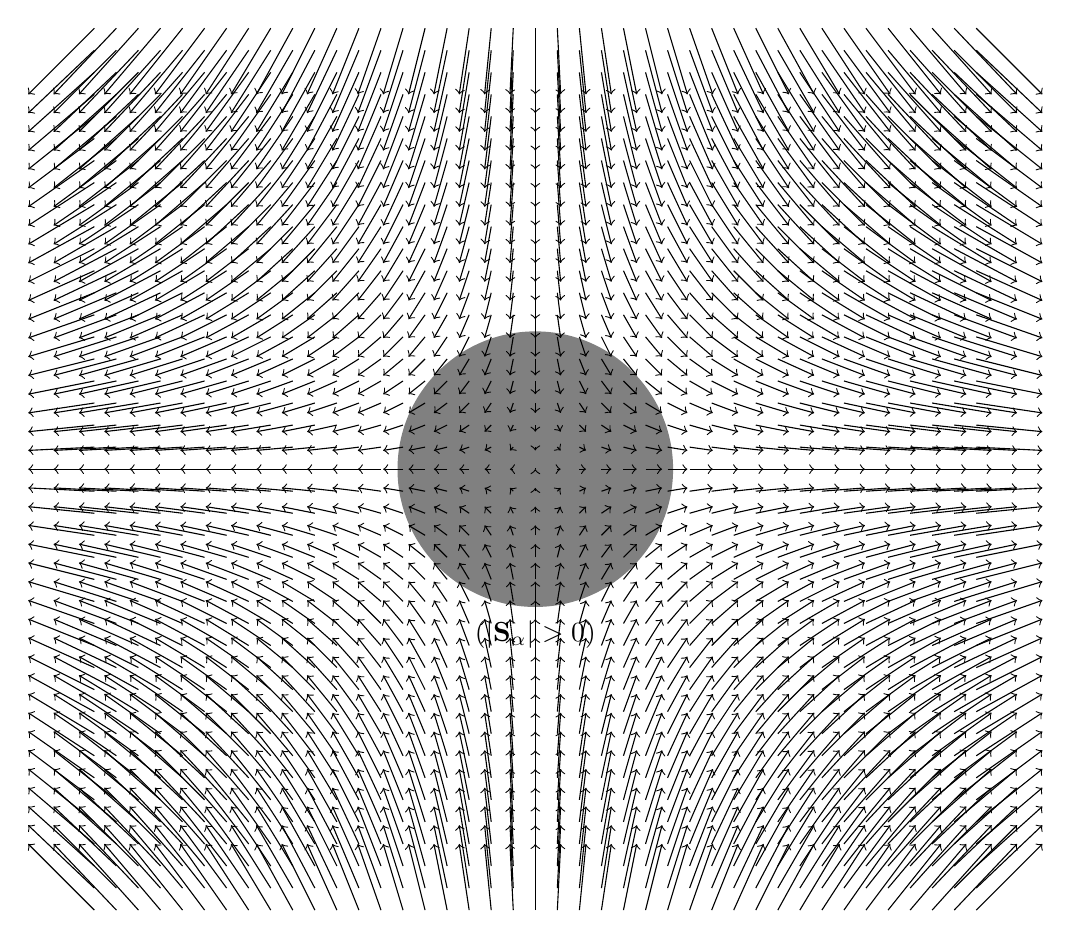
\begin{tikzpicture}[ultra thick,scale=0.7]
        \def\nRows{20}
        \def\nCols{20}
        \fill[gray] (0,0)circle(2.5);
        \foreach \x in {-\nRows,...,\nRows} {
            \foreach \y in {-\nCols,...,\nCols} {
                \pgfmathsetmacro\distance{veclen(\x*0.4, \y*0.4)};
                \pgfmathparse{\distance < 2.5 ? "blue" : "white"}
                \edef\colour{\pgfmathresult};
                \ifthenelse{\equal{\colour}{blue}}{                    
                    \draw[thin,->](\x*0.4,\y*0.4)--++(0.06*\x,-0.06*\y);
                }
            }
        }
        \node (txt) at (0,-3){($|\textbf{S}_\alpha| > 0$)};
    \end{tikzpicture}
    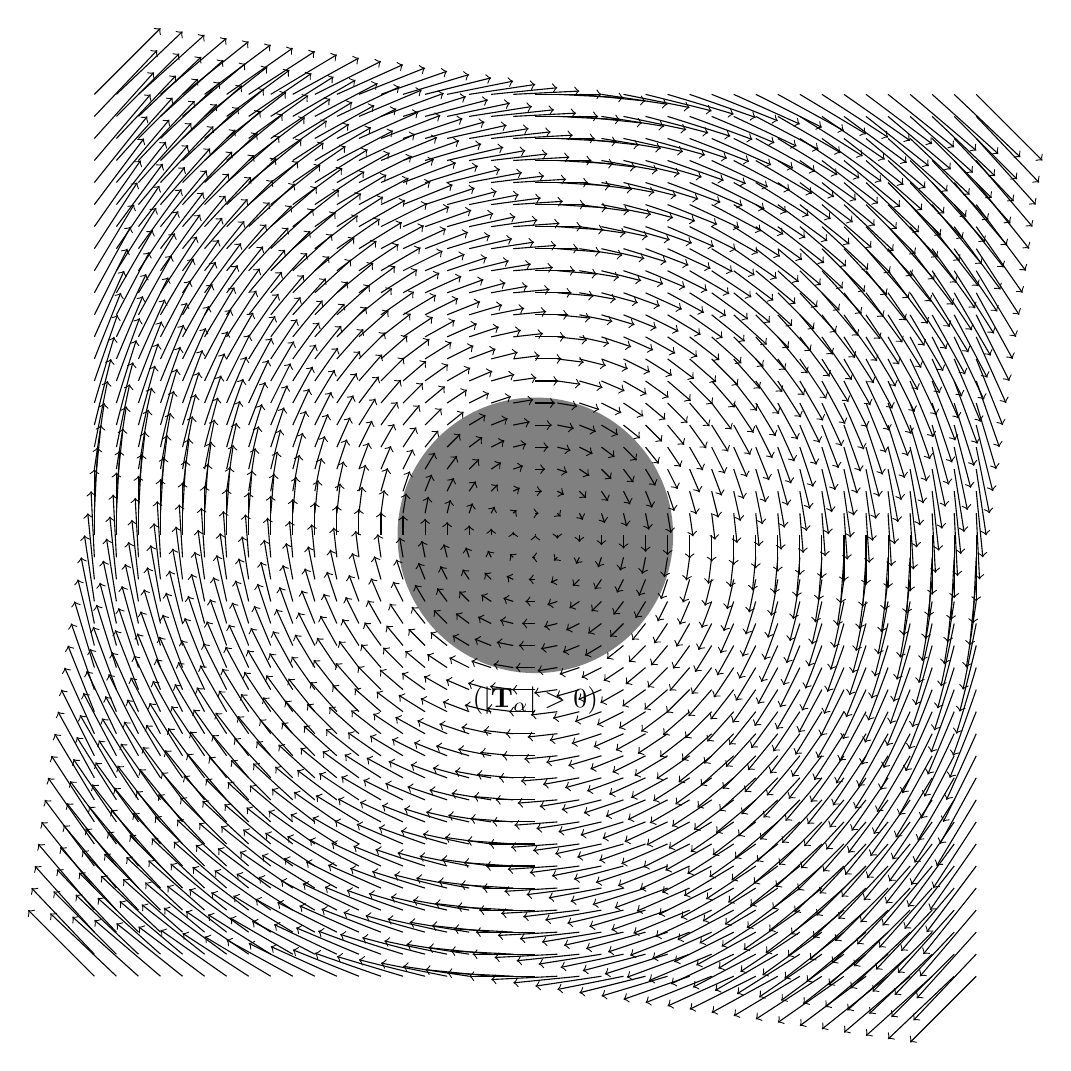
\begin{tikzpicture}[ultra thick,scale=0.7]
        \def\nRows{20}
        \def\nCols{20}
        \fill[gray] (0,0)circle(2.5);
        \foreach \x in {-\nRows,...,\nRows} {
            \foreach \y in {-\nCols,...,\nCols} {
                \pgfmathsetmacro\distance{veclen(\x*0.4, \y*0.4)};
                \pgfmathparse{\distance < 2.5 ? "blue" : "white"}
                \edef\colour{\pgfmathresult};
                \ifthenelse{\equal{\colour}{blue}}{                    
                    \draw[thin,->](\x*0.4,\y*0.4)--++(0.06*\y,-0.06*\x);
                }
            }
        }
        \node (txt) at (0,-3){($|\textbf{T}_\alpha| > 0$)};
    \end{tikzpicture}
    
\begin{tikzpicture}[ultra thick,scale=0.7]
        \def\nRows{20}
        \def\nCols{20}
        \fill[gray] (0,0)circle(2.5);
        \foreach \x in {-\nRows,...,\nRows} {
            \foreach \y in {-\nCols,...,\nCols} {
                \pgfmathsetmacro\distance{veclen(\x*0.4, \y*0.4)};
                \pgfmathparse{\distance < 2.5 ? "blue" : "white"}
                \edef\colour{\pgfmathresult};
                \ifthenelse{\equal{\colour}{blue}}{                    
                    \draw[thin,->](\x*0.4,\y*0.4)--++(-0.06*\x,-0.06*\y);
                }
            }
        }
        \node (txt) at (0,-3){($|D_\alpha| > 0$)};
    \end{tikzpicture}
    \caption{Typical values of moment of momentum. 
    The arrows represent the velocity field inside the droplets with the corresponding value of the moment of momentum tensor.}
\end{figure}

Injecting, $f_2 = \rho_2$ in the second-order moment equation derived in \ref{ap:Moments_equations} we obtain :
\begin{equation}
    \ddt {\textbf{M}_\alpha}=2\textbf{S}_\alpha. 
    \label{eq:dt_M_alpha}
\end{equation}
which is the general form of the second moment of mass conservation equation. 
From \ref{eq:dt_M_alpha} we deduce that the evolution of the distribution of mass of a particle is solely motivated by the stretching of momentum, denoted by $\textbf{S}_\alpha$. 
This implies that the angular momentum (not to be confused with the angular velocity) plays no-role in the evolution of the second moment of the mass distribution. 
Note that if the particle has a constant $\textbf{M}_\alpha$ under change of reference frame, such as for spherical particles where we can write $\textbf{M}_\alpha= \frac{a^2 m_\alpha}{5} \bm\delta$, then the stretching of momentum is null $\textbf{S}_\alpha=0$.
This argument has no restriction on the internal particle motion. 
Additionally, applying the trace operator on both sides of \ref{eq:dt_M_alpha}, yields the interesting relation : $\ddt {\text{tr}(\textbf{M}_\alpha)}=2D_\alpha$.
Therefore, we can state that $\text{tr}(\textbf{M}_\alpha) = \lambda^\alpha_1(t)+\lambda^\alpha_2(t)+\lambda^\alpha_3(t)$, with $\lambda_i^\alpha$ for $i=1,2,3$, being the eigenvalues of $\textbf{M}_\alpha$.
For unreformable particles it is evident that the eigenvalues are not function of time, therefore $\ddt{ \text{tr}(\textbf{M}_\alpha)}=0$.  
Consequently, $D_\alpha$ has the notable property of being null whenever the particle shape remain constant, irrespective of the orientation.
The third invariant of this tensor can be shown to be related to the volume of the particle. 

Now, that we described the shape of the particle through its with the symmetric part of the moment of momentum we might need an equation for the moment of momentum. 
This equation is derived injecting $\textbf{Q}_\alpha = \textbf{P}_\alpha$ in \ref{eq:dt_Q_alpha_tot}, it reads, 
\begin{equation}
    \ddt {\textbf{P}_\alpha}
    = \intO{ \left(
        \rho_2  \textbf{w}_2^0 \textbf{w}_2^0 
        - \bm{\sigma}_2^0
    \right) }
    - \intS{ 
        \gamma \bm\delta_{||}
    }
    + \intS{ \textbf{r}\bm{\sigma}_1^0\cdot \textbf{n}_2} 
    \label{eq:dt_P_alpha}
\end{equation}
The last term on the right-hands side of \ref{eq:dt_P_alpha} represents the first hydrodynamic moment of the force traction on the particle surface.

 

The conservation equation of the angular momentum $\bm{\mu}_\alpha$ is obtained by taking the double contracted product of \ref{eq:dt_P_alpha} with $\bm\epsilon$, which gives the simple expression :
\begin{equation}
    \ddt\bm{\mu}_\alpha
    =  
    % \textbf{t}_\alpha.
    \intS{ \textbf{r} \times \bm{\sigma}_1^0\cdot \textbf{n}_2 }
    \label{eq:dt_mu_alpha}
\end{equation}
Notice that every terms on the RHS of \ref{eq:dt_P_alpha} vanish due to their symmetric nature apart from the shew-symmetric part of the hydrodynamic stress, which is the hydrodynamic torque applied on the particle $\alpha$.
Particularly, the surface tension terms do not appear in the angular momentum balance since $\bm\sigma_I^0 = \gamma (\bm\delta-\textbf{nn})$ is symmetric, which is consistent with the findings of \citet{hesla1993note}. 
As a consequence, the surface tension has no effect on the angular momentum regardless of the particle's shape. 
In the literature it is common to include the torque due to inter-particular interactions in the angular momentum balance, as it is done in \citet{jackson1997locally} and \citet{zhang1997momentum}.
Therefore, we remind the reader that $\bm{\sigma}_0^1$ contains also the short range interaction forces.


Taking the symmetric part of \ref{eq:dt_P_alpha}, yield an equation for the stretching of momentum, which can be written as,
\begin{equation}    
    \ddt{\textbf{S}_\alpha}
    =  \intO{
        (\rho_2\textbf{w}_2^0 \textbf{w}_2^0
        - \bm{\sigma}_2^0)}
        - \intS{\gamma(\bm\delta-\textbf{nn})}
        + \frac{1}{2}\intS{(\textbf{r}\bm\sigma_1^0+ \bm\sigma_1^0\textbf{r})\cdot \textbf{n}}
    \label{eq:dt_S_alpha}
\end{equation}
\tb{introduce the second order derivative here ? }
One might immediately recognize that this equation is in facts an extension to Batchelor’s famous result, 
\begin{equation*}
    \intO{\bm{\sigma}_2^0}
    = \frac{1}{2}\intS{(\textbf{r}\bm\sigma_1^0+ \bm\sigma_1^0\textbf{r})\cdot \textbf{n}}
    - \intS{\gamma(\bm\delta - \textbf{nn})}
\end{equation*}
% \tb{it is also an extension to dolata recent results for teh first and second moment equation }
which has been used widely in stokes flow theory to express the unknown internal stress within solid particles in terms of surface integral, i.e. the stress let $\intS{(\textbf{r}\bm\sigma_2^0+ \bm\sigma_2^0\textbf{r})\cdot \textbf{n}}$.
This relation is the main tools used to express the bulk stress of a suspension, it eventually leads to the computation of the famous Einstein equivalent viscosity upon having an analytical formula for $\intS{(\textbf{r}\bm\sigma_2^0+ \bm\sigma_2^0\textbf{r})\cdot \textbf{n}}$. 
Therefore, the significant aspect of \ref{eq:dt_S_alpha} is that it can be interpreted as a generalized equation for the integrated stress tensor within the volume of the particle.
This will become particularly relevant when determining the total stress of an inertial suspension as it will be mentioned in \ref{sec:averaged_eq}.
On the right-hands side of \ref{eq:dt_S_alpha} we can identify several terms: 
the internal kinetic energy $\intO{\rho_2\textbf{w}_2^0\textbf{w}_2^0 }$; 
the integral of the particle internal stress $\intO{ \bm{\sigma}_2^0
 }$; 
the integral of the surface stress $\intS{ \sigma (\bm\delta- \textbf{nn}) }$; 
and the hydrodynamic stress tensor, $\intS{(\textbf{r}\bm\sigma_2^0+ \bm\sigma_2^0\textbf{r})\cdot \textbf{n}}$ introduced earlier.
Based on \ref{eq:dt_M_alpha} we can infer that the evolution of $\textbf{M}_\alpha$ is driven by the internal kinetic energy and the stresslet.
However, it is being counteracted by surface tension forces and internal stresses which tend to oppose the deformation of the particle. 
Therefore, if the surface tension forces play no role in the linear and angular momentum equation, it does impact the stretching of momentum $\textbf{S}_\alpha$.
As a consequence, the surface tension force impact the hydrodynamic behavior of a particle solely through its action on $\textbf{S}_\alpha$, which is related to the shape of a particle through \ref{eq:dt_M_alpha}.
As remarked by \citet{batchelor1970stress}, since the surface tension force oppose the deformation of a particle, it can be understood as an elastic force. 
Which, as it will be shown in \ref{sec:averaged_eq} has a role on the bulk stress of the suspension. 
% Additionally, note that \ref{eq:dt_S_alpha} can be seen as a formula to reformulate the integral of the internal stress $\pOavg{\bm{\sigma}}$.
Equally, in \ref{ap:moment_derivative} we show how to derive the higher order moment of momentum equations, which can also be viewed as formulas for the higher moments of the internal particle stress distribution. 
It is interesting to mention that in a recent study of \citet{dolata2021faxen} they use energy method and recover the first two moments of momentum equations hidden into another but equivalent form, valid in the stokes flow regime. 


Lastly, by taking the double contracted product of \ref{eq:dt_Q_alpha_tot} with the unit tensor $\bm\delta$, directly yields the scalar equation :
\begin{equation}
    \ddt {D_\alpha}
    = \frac{1}{3}\intO{ \rho_2 \textbf{w}_2^0 \cdot \textbf{w}_2^0}
    + \intO{p_2^0} 
    - \frac{2}{3} \gamma s_\alpha
    + \frac{1}{3}\intS{\textbf{r}\cdot\bm\sigma_1^0\cdot \textbf{n}}
    \label{eq:dt_D_alpha}
\end{equation}
where $s_\alpha = \intS{}$ and we have made use of the explicit form of the Newtonian stresses to highlight the role of the pressure. 
This, corresponds to the isotropic work balance within the particle's volume and surface. 
As a matter of fact, the rate of compression of a particle, denoted by the scalar $D_\alpha$ evolves according to : 
the internal kinetic energy, $\intO{\rho_2 \textbf{w}_2^0 \cdot \textbf{w}_2^0 }$;
the trace of the integral of the hydrodynamic stresses, $\intO{ \text{tr}(\bm{\sigma}_2^0)}$; 
the surface energy $\intS{ \gamma }$; 
and the trace of the hydrodynamic first moment, $\text{tr}(\textbf{M}_\alpha)$.

